%!TEX program = pdflatex
\documentclass[a4paper]{article}
\title{\textbf{Homework 2}}
\author{Wendi Chen}
\date{}
\usepackage{listings}
\usepackage{graphicx} 
\usepackage{indentfirst} 
\begin{document}
\maketitle

\section{Q2: Time Complexity}
In order to implement \emph{Lagrange Interpolation}, we need to calculate the values of $l_{k}(x)$($k$ from $0$ to $n$) first and then use another loop to add them up to get the value at $x$.
Because these two loops are nested, the time complextiy is $O(n^{2})$.
\begin{lstlisting}[language={c++}]
        double ans = 0;
        for(int i = 0;i<n;i++){
            double s = Y[i];
            for(int j = 0;j<n;j++){
                if(j!=i)
                    s *=(x-X[j])/(X[i]-X[j]);
            }
            ans += s;
        }
	return ans;
\end{lstlisting}

For \emph{Newton Interpolation}, there're mainly two steps.
First, we need to use the difference method to calculate the coefficients.
In my implemention, I allocate a $n\times n$ matrix to store intermediate values and execute a two-layer loop for calculation.
This part accounts for a $O(n^{2})$ time complexity.

\begin{lstlisting}[language={c++}]
	for(int i = 1;i<n;i++){
            for(int j = i;j<n;j++){
                table[i][j]=table[i-1][j]-table[i-1][j-1];
            }
        }
\end{lstlisting}

Next, according to the definition of \emph{Newton Interpolation}, calculate the $t$ first and then bring in the coefficients, which also costs a $O(n^{2})$ time complexity. 
\begin{lstlisting}[language={c++}]
	double t = (x-X[0])/h;
        double ans = Y[0];
        for(int i = 1;i<n;i++){
            double ans_k=table[i][i];
            for(int j = 1;j<=i;j++){
                ans_k/=1.0*j;
                ans_k*=1.0*(t-j+1);
            }
            ans+=ans_k;
        }
	return ans;
\end{lstlisting}

So, the overall time complexity is also $O(n^{2})$.

\section{Q3: Drawing and Analysis}

Since the interpolation range is not very large, and the existing points are evenly distributed, we can just divide the interval into 10,000 points and apply the above algorithms to each point. Then, use \textbf{Python} to visualize.

\begin{figure}[!h]
    \centering
    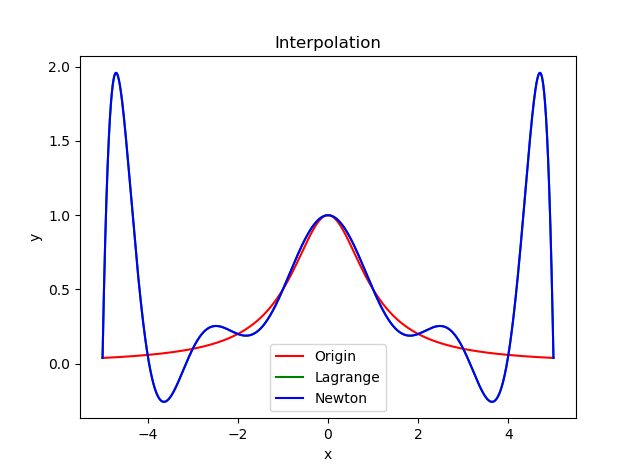
\includegraphics[width=.6\textwidth]{./figures/Figure_1.png}
    \caption{original function and interpolating polynomials}
    \label{fig:Figure_1}
\end{figure}
As the Figure \ref{fig:Figure_1} shows, no matter we use \emph{Lagrange Interpolation} or \emph{Newton Interpolation}, we will get the \textbf{same} interpolating polynomials.
This is predictable.
It can be proved mathematically that the polynomials obtained by \emph{Lagrange interpolation} and \emph{Newton interpolation} are the same after simplification.

Also, the original curve and the interpolation curve intersect at the interpolation point, which is permitted by the base functions we use in these two methods.
However, the interpolation polynomial curve is more undulating than the original curve since we use polynomials to approximate.


\end{document}